\documentclass[12pt]{article}

\usepackage{blindtext} % Package to generate dummy text throughout this template 
\usepackage{amssymb, amsthm, amsmath}

% writing
\usepackage[utf8]{inputenc}
\usepackage{algorithm}
\usepackage[noend]{algpseudocode}
\linespread{1.5}
\usepackage[margin = 1in]{geometry}
\usepackage{microtype} % Slightly tweak font spacing for aesthetics
\usepackage[english]{babel} % Language hyphenation and typographical rules

% tikz
\usepackage{tikz}
\usepackage{pgfplots}
%\usepackage{pgfplotstable}
\pgfplotsset{compat=1.13}
\usetikzlibrary{external}
\tikzexternalize[prefix=external-figures/]

% fig
\usepackage{natbib}
\usepackage{graphicx}
\usepackage{float}
\usepackage{wrapfig}
\usepackage{multicol}

% misc
\usepackage{nomencl}
\usepackage[titletoc, page]{appendix}
\usepackage{multirow}

% caption features
\usepackage{caption}
\usepackage{subcaption}
\usepackage{setspace}
\captionsetup{font={small, stretch=1.25}}
\let\Algorithm\algorithm
\renewcommand\algorithm[1][]{\Algorithm[#1]\setstretch{1.25}}

% ref
\usepackage[pdfpagelabels]{hyperref}
\usepackage{url}
\hypersetup{
    colorlinks=true,
    linkcolor=black,
    urlcolor=black,
    citecolor=black
}
\usepackage[capitalise]{cleveref}
\crefname{appsec}{Appendix}{Appendices}
%\Crefformat{section}{\S#2#1#3}
%\Crefformat{subsection}{\S#2#1#3}
%\Crefformat{subsubsection}{\S#2#1#3}

\setlength{\parindent}{2em}
%\setlength{\parskip}{1.5em}
\graphicspath{ {images/} }

% nomenclature specs
\makenomenclature
\setlength{\nomitemsep}{-\parsep}
\renewcommand{\nomname}{List of Functions, Symbols and Terms}
%% This code creates the groups
% -----------------------------------------
\usepackage{etoolbox}
\renewcommand{\nomgroup}[1]{%
    \item[\bfseries
    \ifstrequal{#1}{T}{Terms}{%
        \ifstrequal{#1}{S}{Symbols}{%
            \ifstrequal{#1}{F}{Functions}{}}%
    }]}
% -----------------------------------------

\newtheorem{mydef}{Definition}
\newcommand{\vect}[1]{\mathbf{#1}}  % vector
\newcommand{\matr}[1]{\mathbf{#1}}  % matrix
\newcommand{\tens}[1]{\mathbf{#1}}  % tensor
\newcommand{\mean}[1]{\overline{#1}}    % mean overline

\title{Report: Solving the Avicaching Problem Faster and Better}
\author{Anmol Kabra, Yexiang Xue and Carla Gomes}
\date{Summer 2017}

\begin{document}
    \pagenumbering{roman}
    \begin{titlepage}
        \maketitle
        \thispagestyle{empty}
    \end{titlepage}
    
    % nomenclature
    \mbox{}
    % symbols
    \nomenclature[S]{$J$}{Number of locations in the dataset}
    \nomenclature[S]{$T$}{Number of time units for which data is available}
    \nomenclature[S]{$n_F$}{Number of features in the dataset $\matr{F}$ (length of $\matr{F}[v][u]$)}
    
    % functions
    \nomenclature[F]{softmax($\cdot$)}{Defined as softmax($z_i$) = $\frac{\exp(z_i)}{\sum_{i} \exp(z_i)}$}
    \nomenclature[F]{reLU($\cdot$)}{Rectified Linear Unit; defined as reLU($z$) = max(0, $z$)}
    \nomenclature[F]{batch-multiply($\cdot$)}{Operates on $m \times n \times p$ and $m \times p \times q$ tensors to give a $m \times n \times q$ tensor.}
    
    % terms
    \nomenclature[T]{Epoch}{One training/testing period; iteration}
    \nomenclature[T]{CPU ``set''}{\textit{All} operations done on the CPU}
    \nomenclature[T]{GPU ``set''}{\textit{Only Matrix/Tensor} operations done on the GPU, rest on the CPU}
    \nomenclature[T]{LP}{Linear Programming}
    \nomenclature[T]{LP Standard Format}{Arrangement of objective function and constraints operated on by library LP solvers - minimize [$\vect{c}^T \vect{x}$]; subject to [$\matr{A} \vect{x} \leq \vect{b}, \, x_i \geq 0$]}
    \nomenclature[T]{Tensor}{Multi-dimensional (usually more than 2 dimensions) array}
    \printnomenclature[1.5in]
    \cleardoublepage
    
    \tableofcontents
    \listoftables
    \listoffigures
    \cleardoublepage
    \pagenumbering{arabic}
    % main body
    \section{Introduction} \label{sec:Introduction}
    Optimizing predictive models on datasets obtained from citizen-science projects can be computationally expensive as these datasets grow in size. Consequently, running models based on Multi-layered Neural Networks, Integer Programming and other optimization routines can become more computationally difficult as the number of parameters increase, despite using the faster Central Processing Units (CPUs) in the market. Incidentally, it becomes difficult for citizen-science projects to scale if the organizers use CPUs to run neural networks, which require extensive tensor operations. However, Graphical Processing Units (GPUs), which offer numerous cores to parallelize computation, can outperform CPUs in computing such predictive models if these models \textit{heavily} rely on large-scale tensor operations []. By using GPUs over CPUs to accelerate computation on a citizen-science project, the model could achieve better optimization in less time, enabling the project to scale.
    
    \subsection{Avicaching}
    Part of the eBird project, which aims to ``maximize the utility and accessibility of the vast numbers of bird observations made each year by recreational and professional bird watchers'' [cite website], Avicaching is a incentive-driven game trying to homogenize the spatial distribution of citizens' (agents') observations \cite{Xue2016Avi1}. Since the dataset of agents' observations in eBird is geographically heterogeneous (concentrated in some places like cities and sparse in others), Avicaching homogenizes the observation set by placing rewards at and attracting agents to under-sampled locations \cite{Xue2016Avi1}. For the agents, collecting rewards increases their `utility' (excitement, fun etc.), while for the organizers, a more homogeneous observation dataset means better sampling and higher confidence in using it to deploy other models. 
    
    To accomplish this task of specifying rewards at different locations based on the historical records of observations, Avicaching would learn how agents change their behavior when a certain sample of rewards were applied to the set of locations, and then redistribute rewards across the locations based on those learned parameters \cite{Xue2016Avi2}. This requirement naturally translates into a predictive optimization problem, implemented using multi-layered neural networks and linear programming.
    
    \subsection{Important Questions}
    Although the previously devised solutions to Avicaching were conceptually effective \cite{Xue2016Avi1, Xue2016Avi2}, using CPUs to solve Mixed Integer Programming and (even) shallow neural networks made the models impractical to scale. Solving the problems faster would have also allowed organizers to find better results (more optimized). These concerns, which form the pivot for our research, are concisely described below.
    
    \subsubsection{Solving Faster} \label{sec:Important Questions - Solving Faster}
    We were interested in using GPUs to run our optimization models because of their capability to accelerate problems based on large tensor operations. Newer generation NVIDIA GPUs, equipped with thousands of CUDA (NVIDIA's parallel computing API) cores \cite{NVIDIA}, could have empowered Avicaching's organizers to scale the game, if the game was computed using simple arithmetic operations on tensors, rather than using conditional logic (see \Cref{sec:Computation Using GPUs}). Since even the faster CPUs - in the range of Intel Core i7 chipsets - are sequential in processing and do not provide as comparable parallel processing\footnote{CPUs often have multiple cores nowadays, but very few compared to what many GPUs have. We use Intel i7-7700K (4 cores) CPU and NVIDIA Quadro P4000 (1792 CUDA cores) for our tests.} as GPUs do, we seek to solve the problem much faster using GPUs. \textbf{But how much faster?}
    
    \subsubsection{Better Results} \label{sec:Important Questions - Better Results}
    The previous model, for learning the parameters in agents' change of behavior on a fixed set of rewards, delivered predictions that differed 26\% from Ground Truth \cite[Table 1]{Xue2016Avi2}. This model was then used to redistribute rewards in a budget. If we could get closer to the Ground Truth, i.e., better learn the parameters for the change, we could redistribute rewards with superior prediction/accuracy. Since the organizers need the \textit{best} distribution of rewards, we will need a set of learned parameters that is closer to the Ground Truth (in terms of Normalized Mean Squared Error \cite[Section 4.2]{Xue2016Avi2}). In a gist, we aim to \textbf{learn the parameters more suitably}, and find the \textbf{best allocation of rewards?}
    
    \subsubsection{Adjusting the Model's Features} \label{sec:Important Questions - Adjusting the Model's Features}
    Once our model starts delivering better results than the previously devised models, one thinks if some characteristics of the model (hyper-parameters such as learning rate) can be changed to get more preferable results (one could also build a better model). While a goal of ``getting better results'' is an unending struggle, there is a trade-off with practicality as these adjustments take time and computation power to test - and we didn't have unlimited resources. Therefore, we asked if one could \textbf{reasonably adjust hyper-parameters to improve performance and optimization.}
    
    \subsection{Computation Using GPUs} \label{sec:Computation Using GPUs}
    // todo
    
    \section{Problem Formulation} \label{sec:Problem Formulation}
    Our models strongly draws from the previous studies \cite{Xue2016Avi1, Xue2016Avi2}, with modifications directed at reducing computation time, as well as getting better results. Since GPUs enable faster computation on tensors, both the Identification and the Pricing Problem are formulated as tensor-based 3-layered and 2-layered neural networks respectively using the Pytorch library \cite{PTDocs}. Recognizing that NVIDIA GPUs easily pair with Pytorch \cite{PTDocs}, accelerating tensor operations using CUDA and cuDNN \cite{cuDNNPaper, NVIDIA}, we aim to maximize parallel operations and minimize thread synchronization.
    
    \subsection{Identification Problem} \label{sec:Identification Problem}
    As discussed in \Cref{sec:Introduction}, the model should learn parameters that caused the change in agents' behavior when a certain set of rewards was applied to locations in the experiment region. Learning those parameters will help us understand how agents behave with a fixed reward distribution, and will enable organizers to redistribute rewards based on that behavior.
    
    Specifically, given datasets $\vect{y_t}$ and $\vect{x_t}$ of agents' visit densities at time $t$, before and after the rewards $\vect{r_t}$ were placed, we want to find weights $\matr{w_1}$ and $\matr{w_2}$ that caused the change from $\vect{x_t}$ to $\vect{y_t}$, considering possible influence from environmental factors $\matr{f}$ and distances between locations $\matr{D}$. Although the original model proposed to learn a single set of weights $\matr{w}$ \cite{Xue2016Avi2}, our proposed model considers two sets of weights $\matr{w_1}$ and $\matr{w_2}$ as it may theoretically result into higher accuracy and lower loss value. Mathematically, the model can be formulated as:
    \begin{equation} \label{eqn:iden_problem}
        \begin{aligned}
            & \underset{\matr{w_1}, \matr{w_2}}{\text{minimize}}
            & & Z_I(\matr{w_1}, \matr{w_2}) = \sum_{t} (\omega_t(\vect{y_t} - \matr{P}(\matr{f}, \vect{r_t}; \matr{w_1}, \matr{w_2})\vect{x_t}))^{2}
        \end{aligned}
    \end{equation}
    where $\omega_t$ is a set of weights (not a learnable parameter) at time $t$ capturing penalties relative to the priority of homogenizing different locations at time $t$. In other words, it highlights if the organizer wishes higher homogeneity at one time unit over another. Elements $p_{u, v}$ of $\matr{P}$ are given as ($\vect{\Theta_i}$ substituted for $\vect{w_i}_v^T$):
    \begin{equation} \label{eqn:puv_equation}
    p_{u, v} = \frac{\exp(\vect{\Theta_2} \cdot \text{reLU} (\matr{\Theta_1} \cdot [d_{u, v}, \vect{f_{u}}, r_{u}]))}{\sum_{u'} \exp(\vect{\Theta_2} \cdot \text{reLU} (\matr{\Theta_1} \cdot [d_{u', v}, \vect{f_{u'}}, r_{u'}]))} = \frac{\exp(\Gamma_{u, v})}{\sum_{u'}\exp(\Gamma_{u', v})} = \text{softmax}(\Gamma_{u, v})
    \end{equation}
    
    To optimize the loss value $Z_I(\matr{w_1}, \matr{w_2})$, the neural network learns the set of weights through multiple epochs of backpropagating the loss using gradient descent. Furthermore, the program preprocesses the dataset to avoid unnecessary sub-epoch iterations and to promote batch operations on tensors.
    
    \subsubsection{Structure of Input Dataset for Identifying Weights} \label{sec:Structure of Input Dataset for Identifying Weights}
    \begin{figure}[!htbp]
        \begin{subfigure}{.64\textwidth}
            \centering
            \includegraphics[width=\linewidth]{weights_input_dataset}
            \caption{A Tensor representing the Input Dataset $\tens{F}$}
            \label{fig:A Tensor representing the complete Input Dataset}
        \end{subfigure}
        \begin{subfigure}{.35\textwidth}
            \centering
            \includegraphics[width=\linewidth]{zoomup_Fuv}
            \caption{Contents of $\tens{F}[v][u]$: This vector (length $n_F$) contains quantified causes for the change in agents' behavior from $\matr{x_t}$ to $\matr{y_t}$}
            \label{fig:Zoomed-in contents of Fvu}
        \end{subfigure}
        \caption{Visual representation of the Input Dataset}
        \label{fig:Visual representation of the Input Dataset}
    \end{figure}
    Since preprocessing the dataset reduces data operations during model execution, the input dataset, comprising of distance between locations $\matr{D}$, environmental features $\vect{f}$ and given rewards $\vect{r_t}$ (all normalized), is built into a tensor (\Cref{fig:A Tensor representing the complete Input Dataset}) such that operations can be performed on batches of slices $\tens{F}[v]$.
    
    Another advantage of building the dataset as a tensor comes with the Pytorch library, which provides convenient handling and transfer of tensors residing on the Main Memory and GPUs' internal global memory \cite{PTDocs}. \Cref{alg:Constructing the Input Dataset} describes the steps to construct this dataset.
    \begin{algorithm}
        \caption{Constructing the Input Dataset} \label{alg:Constructing the Input Dataset}
        \begin{algorithmic}[1]
            \Function{Build-Dataset}{$\matr{D}, \matr{f}, \matr{r_t}$}
            \State $\matr{D} \gets \Call{Normalize}{\matr{D}}$\Comment{$\matr{D}[u][v]$ is the distance between locations $u$ and $v$}
            \State $\vect{f} \gets \Call{Normalize}{\mathbf{f}, axis = 0}$\Comment{$\mathbf{f}[u]$ is a vector of env. features at location $u$}
            \State $\vect{r_t} \gets \Call{Normalize}{\vect{r_t}, axis = 0}$\Comment{$\vect{r_t}[u]$ is the reward at location $u$}
            \For{$v = 1, 2, \dots, J$}
                \For{$u = 1, 2, \dots, J$}
                    \State $\tens{F}[v][u] \gets [\matr{D}[v][u], \vect{f}[u], \vect{r_t}[u]]$ \Comment{As depicted in \Cref{fig:Zoomed-in contents of Fvu}}
                 \EndFor
            \EndFor
            \State \Return $\matr{F}$
            \EndFunction
        \end{algorithmic}
    \end{algorithm}

    \subsubsection{Minimizing Loss for the Identification Problem} \label{sec:Minimizing Loss for the Identification Problem}
    As shown in \Cref{fig:Neural network designed for the Identification Problem}, the neural network is made of 3 fully connected layers - the input layer, the hidden layer with rectified Linear Units (reLU), and the output layer with softmax$(\cdot)$ function units. The network can also be visualized as a stack of 1-dimensional layers (\Cref{fig:Side view of the network}), with the softmax$(\cdot)$ calculated on the stack's output.
    \begin{figure}[!htbp]
        \centering
        \begin{subfigure}{\textwidth}
            \centering
            \includegraphics[width=\textwidth]{weights_net}
            \caption{3-dimensional View of the Network Slice, Taking in $\matr{F}[v]$}
            \label{fig:3-dimensional view of the network slice taking in Fv}
        \end{subfigure}
        \begin{subfigure}{.75\textwidth}
            \centering
            \includegraphics[width=\textwidth]{weights_net_side}
            \caption{Side View of the Network: Output of one such cross-section is $p_{u_i, v}$}
            \label{fig:Side view of the network}
        \end{subfigure}
        \caption{Neural Network Designed for the Identification Problem}
        \label{fig:Neural network designed for the Identification Problem}
    \end{figure}

    It is important to clarify that the network in \Cref{fig:3-dimensional view of the network slice taking in Fv}, which takes in $\matr{F}[v]$ as shown, is a slice of the original network, which takes in the complete tensor $\matr{F}$ and computes the complete result $\matr{P}^{T}$  per iteration of $t$. In other words, the input and the hidden layers are 3-dimensional, and the output layer is 2-dimensional. Since it is difficult to visualize the complete network on paper, slices of the network are depicted in \Cref{fig:3-dimensional view of the network slice taking in Fv}. \Cref{alg:Algorithm for the Identification Problem} details the steps for learning the parameters $\matr{w_1}$ and $\matr{w_2}$ based on \Cref{eqn:iden_problem,eqn:puv_equation}.
    
    \begin{algorithm}
        \caption{Algorithm for the Identification Problem} \label{alg:Algorithm for the Identification Problem}
        \begin{algorithmic}[1]
            \State $\matr{w_1} \gets \Call{Random}{\;(J,n_F,n_F)\;}$\Comment{$\matr{w_1}$ has dimensions $J \times n_F \times n_F$}
            \State $\matr{w_2} \gets \Call{Random}{\;(J,n_F,1)\;}$\Comment{$\matr{w_2}$ has dimensions $J \times n_F \times 1$}
            \For{$e = 1, 2, \dots, \text{Epochs}$}
                \State $loss \gets 0$
                \For{$t = 1, 2, \dots, T$}
                    \State $\matr{F} \gets \Call{Build-Dataset}{\matr{D}, \matr{f}, \matr{r}[t]}$\Comment{Defined in Algorithm \Cref{alg:Constructing the Input Dataset}}
                    \State $\matr{H} \gets  \text{reLU}(\Call{Batch-Multiply}{\matr{F}, \matr{w_1}})$
                    \State $\matr{O} \gets \text{softmax}(\Call{Batch-Multiply}{\matr{H}, \matr{w_2}})$
                    \State $\matr{P} \gets \matr{O}^T$
                    \State $loss \gets loss + (\omega(\matr{y}[t] - \matr{P} \cdot \matr{x}[t]))^2$
                \EndFor
                \State $\Call{Gradient-Descent}{loss, \matr{w_1}, \matr{w_2}}$
                \State $\matr{w_1}, \matr{w_2} \gets \Call{Update-Using-Gradients}{\matr{w_1}, \matr{w_2}}$
                \State $\Call{Log-Info}{e, loss}$
            \EndFor
        \end{algorithmic}
    \end{algorithm}
    
    \subsection{Pricing Problem} \label{sec:Pricing Problem}
    After learning the set of weights $\matr{w_1}$ and $\matr{w_2}$ highlighting the change in agents' behavior to collect observations, the Pricing Problem aims to redistribute rewards to the all locations such that the predicted behavior of agents influenced by the new set of rewards is homogeneous. Thus, given a budget of rewards $\mathcal{R}$, this optimization problem can be expressed as:
    \begin{equation} \label{eqn:pricing_problem}
        \begin{aligned}
            & \underset{\vect{r}}{\text{minimize}}
            & & Z_P(\vect{r}) = \frac{1}{n}\lVert \vect{y} - \mean{\vect{y}} \rVert\\
            & \text{subject to}
            & & \vect{y} = \matr{P}(\matr{f}, \vect{r}; \matr{w_1}, \matr{w_2}) \, \vect{x}\\
            &&& \sum_{i} r_i \leq \mathcal{R}\\
            &&& r_i \geq 0
        \end{aligned}
    \end{equation}
    where elements of $\matr{P}$ are defined as in \Cref{eqn:puv_equation}.
    
    To allocate the rewards $\vect{r}$ optimally, the calculations for the pricing problem are akin to that for the Identification Problem (see \Cref{sec:Identification Problem}). However, since only 1 set of rewards need to be optimized, we use an altered 2-layer (input and output layers) network instead of the 3-layered network used for the Identification Problem. While \Cref{eqn:pricing_problem} looks like a typical Linear Programming problem, only a part of the formulation uses LP to constrain the rewards. We calculate $\matr{P}$ using a 2-layered network that minimizes the loss function $Z_P(\vect{r})$ using gradient descent, and constrain the rewards using linear programming. Fundamental processes are described below, whereas specific implementation details, with code optimizations and more data preprocessing, are described in \Cref{app:Implementation}.
    
    \subsubsection{Input Dataset for Finding Rewards}
    Since it is the set of rewards $\vect{r}$ that need to be optimized, they must serve as the ``weights'' of the network (``weights'' here refer to the weighted edges of this network and not to the set of calculated weights $\matr{w_1}$ and $\matr{w_2}$). Therefore, the rewards $\vect{r}$ are no longer fed into the network but are its characteristic. Instead, the calculated weights $\matr{w_1}$ are fed into the network, and are ``weighted'' by the rewards.
    
    The observation density datasets, $\matr{x}$ and $\matr{y}$, are also aggregated for all agents such that they give information in terms of locations $u$ only. This is also why rewards vector $\vect{r}$ does not depend on $t$ - we want a generalized set of rewards for all time $t$ per location $u$. Therefore, the algorithm for constructing $\matr{F}$ (see \Cref{sec:Structure of Input Dataset for Identifying Weights}) is same as \Cref{alg:Constructing the Input Dataset} but with a change - $\vect{r_t}$ replaced by $\vect{r}$.
    
    \subsubsection{Calculating Rewards} \label{sec:Calculating Rewards}
    \Cref{alg:Solving the Pricing Problem} for finding $\matr{P}$ is very similar to \Cref{alg:Algorithm for the Identification Problem}'s first few steps but without any epochs of $t$. Also, since the model would predict $\vect{y}$, it does not need labels $\vect{y}$ as a dataset. Although \Cref{alg:Solving the Pricing Problem}'s logic flow may seem arcane, it is straight-forward - as displayed in \Cref{fig:Logic Flow of Algorithm Pricing Problem}.
    \begin{figure}[!htbp]
        \centering
        \includegraphics[width=\textwidth]{logic_alg_pricing}
        \caption{Logic Flow of \Cref{alg:Solving the Pricing Problem}}
        \label{fig:Logic Flow of Algorithm Pricing Problem}
    \end{figure}
    \begin{algorithm}
        \caption{Solving the Pricing Problem} \label{alg:Solving the Pricing Problem}
        \begin{algorithmic}[1]
            \Function{Forward}{$\matr{D}, \matr{f}, \vect{r}, \matr{w_1}, \matr{w_2}, \vect{x}$}
                \State $\matr{F} \gets \Call{Build-Dataset}{\matr{D}, \matr{f}, \vect{r}}$\Comment{Defined in  \Cref{alg:Constructing the Input Dataset}}
                \State $\matr{O}_1 \gets \text{reLU}(\Call{Batch-Multiply}{\matr{F}, \matr{w_1}})$
                \State $\matr{O}_2 \gets \text{softmax}(\Call{Batch-Multiply}{\matr{O}_1, \matr{w_2}})$
                \State $\matr{P} \gets \matr{O}_2^T$
                \State $\vect{y} \gets \matr{P} \cdot \vect{x}$
                \State \Return $\lVert \vect{y} - \mean{\vect{y}} \rVert / J$
            \EndFunction
            \vspace*{-.7\baselineskip}\Statex\hspace*{\dimexpr-\algorithmicindent-2pt\relax}\rule{\textwidth}{0.1pt}%
            \Statex\hspace*{-\algorithmicindent}\textbf{Main Script}%
            \vspace*{-.6\baselineskip}\Statex\hspace*{\dimexpr-\algorithmicindent-2pt\relax}\rule{\textwidth}{0.1pt}% horizontal rule
            \State $\vect{r} \gets \Call{Random}{\;(J)\;}$\Comment{$\vect{r}$ has dimensions $J$}
            \State $loss \gets \Call{Forward}{\matr{D}, \matr{f}, \vect{r}, \matr{w_1}, \matr{w_2}, \vect{x}}$
            \For{$e = 1, 2, \dots, \text{Epochs}$}
                
            \State $\Call{Gradient-Descent}{loss, \vect{r}}$
            \State $\vect{r} \gets \Call{Update-Using-Gradients}{\vect{r}}$
            \State $\vect{r} \gets \Call{LP}{\vect{r}, \mathcal{R}}$\Comment{LP($\cdot$) explained in \Cref{sec:Constraining Rewards}}
            \State $loss \gets \Call{Forward}{\matr{D}, \matr{f}, \vect{r}, \matr{w_1}, \matr{w_2}, \vect{x}}$
            \State $\Call{Log-Best-Rewards}{loss, \vect{r}}$\Comment{Record $\vect{r}$ with the lowest $loss$ yet}
            \EndFor
        \end{algorithmic}
    \end{algorithm}

    \subsubsection{Constraining Rewards} \label{sec:Constraining Rewards}
    After updating the rewards, the program constrains them using LP($\cdot$) such that $\sum_{i}r_i \leq \mathcal{R}$ and $r_i \geq 0$. To do so, the LP($\cdot$) finds another set of rewards $\vect{r'}$ such that the absolute difference between new and old rewards ($\sum_{i}|r'_i - r_i|$) is minimum. The mathematical formulation is given in \Cref{eqn:lp_math_constrain_rewards}, which was implemented using SciPy's Optimize Module \cite{SCPOptimizeDocs}. Since the module supports a standard format for doing linear programming, \Cref{eqn:lp_code_constrain_rewards} is used (see \Cref{app:Implementation}), which is mathematically equivalent to \Cref{eqn:lp_math_constrain_rewards}.
    \begin{multicols}{2}
        \begin{equation} \label{eqn:lp_math_constrain_rewards}
            \begin{aligned}\\
                & \underset{\vect{r'}}{\text{minimize}}
                & & \sum_{i}|r'_i - r_i|\\
                & \text{subject to}
                & & \sum_{i}r'_i \leq \mathcal{R}\\
                &&& r_i \geq 0\\ \\
            \end{aligned}
        \end{equation}\break
        \begin{equation} \label{eqn:lp_code_constrain_rewards}
            \begin{aligned}
                & \underset{[\vect{r'}, \vect{u}]}{\text{minimize}}
                & & \sum_{i} u_i\\
                & \text{subject to}
                & & r'_i - r_i \leq u_i\\
                &&& r_i - r'_i \leq u_i\\
                &&& \sum_{i} r'_i \leq \mathcal{R}\\
                &&& r'_i, u_i \geq 0
            \end{aligned}
        \end{equation}
    \end{multicols}
    
    We make a tradeoff by constraining rewards using LP instead of Mixed Integer Programming, which the previous study used \cite{Xue2016Avi2}. The tradeoff exists between decreasing the computation time and loosening integer constraints on each reward value. While model-learned integer rewards have worked in real-life testing also \cite{Xue2016Avi2}, we cannot say if allowing non-integer values in rewards would produce better results in real-life, corresponding to the model's prediction. In other words, we can't ensure the predicted rewards' effectiveness in ground testing before \textit{actually} deploying them in the game. Nevertheless, we can estimate how good the predictions can be compared to several baseline indicators. These baseline sets are elaborated in \Cref{sec:Pricing Problem-Optimizing the Original Dataset}.
    
    \section{Experiment Specifications} \label{sec:Experiment Specifications}
    We define GPU Speedup as:
    \begin{mydef} \label{def:GPU Speedup}
        GPU Speedup: Ratio of model's \underline{execution} time with GPU ``set'' and that with CPU ``set''. The script's data preprocessing runtime is ignored, but the time taken to transfer data from CPU to GPU is included in calculating GPU ``set'' time elapsed. (Speedup = $\frac{CPU-time}{GPU-time\; +\; Transfer-time}$)
    \end{mydef}

    To test both our models, we conducted several tests for optimization and GPU Speedup. After initializing all parameters randomly (with specific seeds for reproduction and uniformity between tests), the models were run for 1000 or 10000 epochs depending on the complexity of the model.
    
    \subsection{Datasets} \label{sec:Datasets}
    We conducted two types of tests: \textbf{optimization tests on original datasets} and \textbf{GPU Speedup tests on randomly generated datasets}. Data was loaded as Floating Point 32 (FP32) units, but was stored with less precision (up to 15 significant figures) to reduce secondary memory usage.
    
    For the GPU Speedup runs, two random datasets of 173 time units ($T$) were generated beforehand using NumPy (without any seed):
    \begin{enumerate} 
        \item 116 locations - for Identification Problem
        \item 232 locations - for Pricing Problem
    \end{enumerate}
    
    We used more locations for the Pricing Problem's model because its 2-layered network was less complex and time consuming than Identification Problem's 3-layered network. Additionally, this decision emerged after initially testing the Pricing Problem on 116 locations, which did not help us identify the trend (more in \Cref{sec:PriProbRes - GPU}). We believe that speedup tests on original datasets would give similar results, though we used randomly generated datasets because it was easier to scale and build random datasets of different batch-sizes for testing. The models were timed for the executed operations in a neural network and the LP, including transfer times of tensors between the RAM and GPU's internal memory. Time taken for preprocessing was ignored. 
    
    \subsection{Test-Machine Configuration} \label{sec:Test-Machine Configuration}
    Hardware specifications and software versions used for the experiments are listed in \Cref{tab:Hardware Specifications and Software Versions Used for Experiments}. We restricted (not eliminated) extraneous computing usage by background processes on the test-machine by switching off X (Graphical User Interface for Ubuntu OS) and performing tests in CLI (Command Line Interface), and ending user processes. However, we should point out that other experiments can give varying runtimes (\Cref{sec:Results}), which may differ based on other running processes and threads. However, one should obtain similar GPU Speedup results when repeating the experiments.
    \begin{table}[!htbp]
        \centering
        \caption{Hardware Specifications and Software Versions Used for Experiments}
        \label{tab:Hardware Specifications and Software Versions Used for Experiments}
        \begin{tabular}{|c|c|}
            \hline
            \multicolumn{2}{c}{\textbf{Hardware}}\\
            \hline
            \textbf{Type} & \textbf{Unit/Specs}\\
            \hline
            Desktop & Dell Precision Tower 3620\\
            CPU & Intel Core i7-7700K\\
            RAM & 16GB\\
            GPU & NVIDIA Quadro P4000\\
            \hline
        \end{tabular}\quad
        \begin{tabular}{|c|c|}
            \hline
            \multicolumn{2}{c}{\textbf{Software}}\\
            \hline
            \textbf{Library/Package} & \textbf{Version}\\
            \hline
            Ubuntu OS & 16.04.2 LTS\\
            CUDA & 8.0\\
            cuDNN & 5.1.10\\
            MKL & 2017.0.3\\
            Python & 2.7.13 (Anaconda)\\
            Pytorch & 0.1.12\textunderscore2\\
            NumPy & 1.12.1\\
            SciPy & 0.19.0\\
            \hline
        \end{tabular}
    \end{table}
    
    \paragraph{GPU ``set'' and CPU ``set'' Clarification} By GPU ``set'' we mean \textit{distributing} operations in the scripts between CPU and GPU, while by CPU ``set'' we mean that the operations were executed \textit{only} on the CPU. Since GPUs are inferior than CPUs at handling most operations other than simple arithmetic matrix ones due to parallelism (see \Cref{sec:Computation Using GPUs}), we used - and recommend using - both the CPU and the GPU in the former case (GPU ``set'') to handle operations each is superior at. However, since the models in \Cref{alg:Algorithm for the Identification Problem,alg:Solving the Pricing Problem} (not the full scripts) are primarily arithmetic operations on  tensors, it is clear that they were executed on the GPU when it was ``set'' and on the CPU when the CPU was ``set''. Other than this optimization, we did not specifically design any parallelized algorithm for either configurations, relying on the Pytorch's and NumPy-SciPy's inbuilt implementation.
    
    \subsection{Algorithm Choice} \label{sec:Algorithm Choice}
    On the algorithm side, we used Adam's algorithm for \textsc{Gradient-Descent}($\cdot$), after testing performances of several algorithms\footnote{Pytorch lets you choose the corresponding function/module} including but not limited to Stochastic Gradient Descent (SGD) \cite{SGD}, Adam's Algorithm \cite{Adam} and Adagrad \cite{Adagrad}. In \Cref{sec:Results} (Results), we only discuss and show tests using the Adam's algorithm, since it was found to work best with both models over all test runs.
    
    \subsection{Running the Identification Problem's Model} \label{sec:Running the Identification Problem's Model}
    \subsubsection{Optimizing the Original Dataset} \label{sec:Identification Problem-Optimizing the Original Dataset}
    The 3-layered neural network was run for 10000 epochs on the original dataset, which was split 80:20 for training and testing sets, with different learning rates = $\{10^{-2}, 10^{-3}, 10^{-4}, 10^{-5}\}$. Since we were aiming for optimization, we ran multiple tests (5 different seeds with each learning rate) of the model only with the GPU ``set''.
    
    To compare this model's optimization results with other model structures, the previously studied 2-layered network \cite{Xue2016Avi2} and a 4-layered neural network were used. The 4-layered network had another hidden layer with reLU, equivalent to the hidden layer in the current 3-layered network in \Cref{fig:3-dimensional view of the network slice taking in Fv}. The results from the 2-layered network were obtained from the previous study, and those from the 4-layered network were attained on the same original dataset with same parameter values (learning rates, epochs etc.).
    
    \subsubsection{Testing GPU Speedup on the Random Dataset} \label{sec:Identification Problem-Testing GPU Speedup on the Random Dataset}
    After generating a random dataset and splitting it 80:20 for training and testing to predict performance on the original dataset, we ran our 3-layered model with different batch-sizes $T = 17, 51, 85, 129, 173$ ($J = 116$) and different seeds with both GPU and CPU ``set'', logging the elapsed time for model execution. The total time elapsed was averaged for a batch-size on a device, which were used to generate scatter/line plots (see \Cref{sec:IdProbRes - GPU}).
    
    \subsection{Running the Pricing Problem's Model} \label{sec:Running the Pricing Problem's Model}
    \subsubsection{Optimizing the Original Dataset} \label{sec:Pricing Problem-Optimizing the Original Dataset}
    After obtaining the set of weights $\matr{w_1}$ and $\matr{w_2}$ optimized using different seeds, we tested to find the best rewards (with the lowest loss - \Cref{eqn:pricing_problem}) with random $\vect{r}$ initiation. To obtain the best rewards, the model was run on all sets of weights obtained from the Identification Problem for 1000 epochs with different learning rates. In search for the best rewards with the minimum loss, we took this approach:
    \begin{enumerate}
        \item Run differently seeded rewards on all sets of weights (obtained from the Identification Problem) and identify a set of weights which performed better than the others (low $Z_I$ - \Cref{eqn:pricing_problem}) on average. The learning rate was fixed to $10^{-3}$ in this case.
        \item Use that set of weights to run a number of tests with varying seeds and learning rates = $\{10^{-2}, 5 \times 10^{-3}, 10^{-3}, 5 \times 10^{-4}, 10^{-4}, 5 \times 10^{-5}, 10^{-5}\}$, and choose the rewards which gave the lowest loss value $Z_I$ anytime during execution.\footnote{This means that we selected the rewards before completion if the loss at that epoch was lower than that in the end.} 
    \end{enumerate}

    Two sets of rewards were tested for loss values as baseline comparisons to our model - a randomly generated set, and another with elements inversely proportional to the number of visits at each location. While the former was a random baseline, the latter captured the idea of allocating higher rewards to relatively under-sampled locations. The best loss values were compared for all tests with the baselines.
    
    \subsubsection{Testing GPU Speedup on the Random Dataset} \label{sec:Pricing Problem-Testing GPU Speedup on the Random Dataset}
    Initially, we ran the Pricing Problem's model with different batch-sizes $J = 11, 35, 55, 85, 116$ ($T = 173$) and different seeds with both GPU and CPU ``set''. Since we couldn't find a clear trend, we tested on more locations $J = 145, 174, 203, 232$.
    
    We relied on SciPy's Optimize Module to solve our LP sub-problem (see \Cref{sec:Constraining Rewards}) because Pytorch does not provide a GPU-accelerated Simplex LP solver. Since SciPy's implementation does not utilize the GPU, we expected the LP problem to be executed on the CPU and thus deliver equal runtimes in both GPU and CPU ``set'' configurations.
    
    \section{Results} \label{sec:Results}
    \subsection{Identification Problem's Results} \label{sec:Identification Problem's Results}
    \subsubsection{Optimization Results} \label{sec:IdProbRes - Optimization}
    Running the 3-layered network with the GPU ``set'' with different learning rates on different seeds (to calculate average performance of each learning rate) for 10000 epochs showed that the model was performing constantly giving lower loss values ($Z_I$ - \Cref{eqn:iden_problem}) with learning rate = $10^{-3}$. 
    
    We observed that higher learning rates ($>10^{-2}$) could only decrease the loss function to a limit, after which the updates in the weights caused the loss function to oscillate and increase. This phenomena is exemplified in \Cref{fig:Test Loss Plots of Different Learning Rates to Find Weights}, which are plots of different models with the same seed but different learning rates. On the other side of $10^{-3}$, lower learning rates took too long to train. Runtime for the model on 10000 epochs was 1232.56 seconds (average over 20 runs = 5 seeds $\times$ 4 learning rates), and models with learning rates less than $10^{-3}$ did not perform better than those with learning rate = $10^{-3}$ on \textit{any} run. Although the decrease in test losses were constant for learning rates less than $10^{-3}$, we feel that they may be computationally expensive and temporally inconvenient to train.
    \begin{table}[!htbp]
        \centering
        \caption[Loss Values Calculated for Different Models for Identification Problem]{Loss Values Calculated for Different Models for Identification Problem: For both the 3- and the 4-layered models, learning rate = $10^{-3}$ outperformed other learning rates. Consequently, that learning rate is used in comparison with other models in \Cref{fig:Comparison of Loss Values from Different Models of the Identification Problem}.}
        \label{tab:Loss Values Calculated for Different Models for Identification Problem}
        \begin{tabular}{c | c | c}
            \hline
            \multirow{2}{*}{\textbf{Learning Rate}} & \multicolumn{2}{c}{\textbf{Average Test Loss Values}} \\
            & 3-layered & 4-layered\\
            \hline
            $10^{-2}$ & 0.168 $\pm$ 0.068 & 0.494 $\pm$ 0.083\\
            $10^{-3}$ & \textbf{0.119 $\pm$ 0.016} & \textbf{0.228 $\pm$ 0.048}\\
            $10^{-4}$ & 0.151 $\pm$ 0.040 & 0.237 $\pm$ 0.067\\
            $10^{-5}$ & 0.212 $\pm$ 0.040 & 0.320 $\pm$ 0.067\\
            \hline
        \end{tabular}
    \end{table}
    
    \begin{figure}[!htbp]
        \centering
        \includegraphics[width=16cm, height=10cm]{test_losses_diff_lr_plot}
        \caption{Test Loss Plots of Different Learning Rates to Find Weights}
        \label{fig:Test Loss Plots of Different Learning Rates to Find Weights}
    \end{figure}
    \begin{figure}[!htbp]
        \centering
        \begin{minipage}{.48\textwidth}
            \centering
            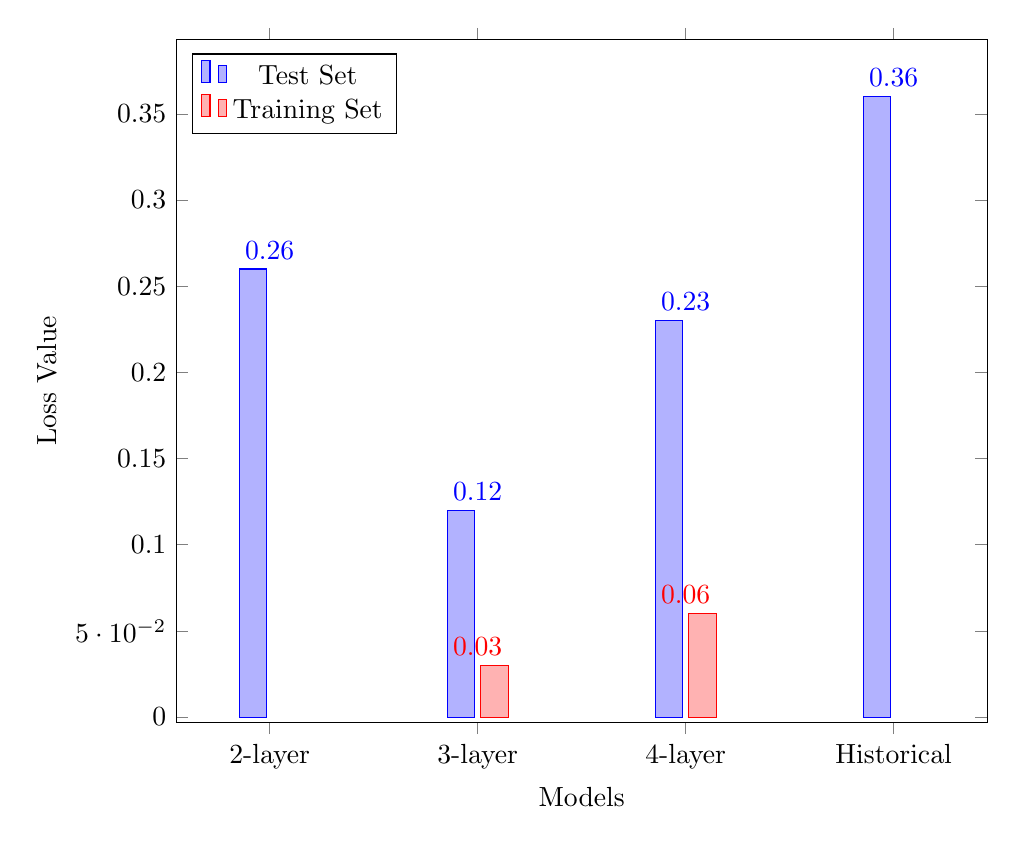
\begin{tikzpicture}
                \begin{axis}[
                    ybar,
                    width=.98\textwidth,
                    enlarge x limits=0.15,
                    legend style={at={(0.02,0.98)},
                        anchor=north west,legend columns=1},
                    ylabel={Loss Value},
                    symbolic x coords={2-layer,3-layer,4-layer, Historical},
                    xtick=data,
                    nodes near coords,
                    nodes near coords align={vertical},
                    every node near coord/.style={/pgf/number format/fixed},
                    xlabel={Models},
                ]
                \addplot coordinates {(2-layer,0.26) (3-layer,0.12) (4-layer,0.23) (Historical, 0.36)};% test set
                \addplot coordinates {(3-layer,0.03) (4-layer,0.06)};% training set
                \legend{Test Set,Training Set}
                \end{axis}
            \end{tikzpicture}
            \caption[Comparison of Loss Values from Different Models of the Identification Problem]{Comparison of Loss Values from Different Models of the Identification Problem: Loss values for the training set are inevitably lower than that for the test set, which should be the basis for comparison}
            \label{fig:Comparison of Loss Values from Different Models of the Identification Problem}
        \end{minipage}\hfill
        \begin{minipage}{.48\textwidth}
            \centering
            \includegraphics[width=\textwidth]{weights_map_plot_3}
            \caption[Predicted Probabilities of Agents Visiting Each Location Plotted on a Map (Latitude, Longitude) Representing Tompkins and Cortland Counties, NY]{Predicted Probabilities of Agents Visiting Each Location Plotted on a Map (Latitude, Longitude) Representing Tompkins and Cortland Counties, NY: Dark dots represent high prediction of visits. This can be compared to the plots for the 2-layered network and other models \cite[Figure 3]{Xue2016Avi2}.}
            \label{fig:Predicted Probabilities of Agents Visiting Each Location Plotted on a Map}
        \end{minipage}
    \end{figure}

    Observing that the average test loss values of learning rate = $10^{-3}$ is the lowest, we compare its results with the previous study's 2-layered network, historical data \cite[Table 1]{Xue2016Avi2}, and the 4-layered network with learning rate = $10^{-3}$ (see \Cref{sec:Identification Problem-Optimizing the Original Dataset}). As depicted in \Cref{fig:Comparison of Loss Values from Different Models of the Identification Problem}, our 3-layered neural network outperformed the previous 2-layered model by \textbf{0.14 units (14\% more closer to Ground Truth - $\matr{y}$)} \cite[Table 1]{Xue2016Avi2}, and also produced much better results (12\% more closer to Ground Truth) than the 4-layered model.
    
    We also generated the predicted probabilities of the agents in the Test Set, visiting each location ($\matr{P}\matr{x}$), and plotted it onto maps marked by the locations' latitudes and longitudes. \Cref{fig:Predicted Probabilities of Agents Visiting Each Location Plotted on a Map} shows such a plot generated by the 3-layered network, where each dot represents a location.
    
    To check if the model was overfitting at learning rate = $10^{-3}$, we plotted loss values at the end of each epoch for all tests. Although there remained $\approx$ 9\% difference (0.09 loss units) in the values of training and testing set, the 3-layered model was not drastically overfitting as an average \textit{end} difference of $8.76 \pm 1.59$\% persisted for many epochs, instead of increasing and tuning more to the training set. Even though one would expect overfitting with more tuned parameters, the 4-layered model also  produced an average \textit{end} difference of $16.77 \pm 4.73\%$, which persisted during the run. \Cref{fig:Train & Test Loss Values' Plots of Different Models} shows the results of a randomly selected experiment with plots of loss values at each epoch for the both networks.
    \begin{figure}[!htbp]
        \centering
        \begin{subfigure}{.49\textwidth}
            \centering
            \includegraphics[width=\textwidth]{weights_train_test_loss_3_plot}
            \caption{Plot for 3-layered Model}
            \label{fig:Plot for 3-layered Model}
        \end{subfigure}
        \begin{subfigure}{.49\textwidth}
            \centering
            \includegraphics[width=\textwidth]{weights_train_test_loss_4_plot}
            \caption{Plot for 4-layered Model // todo}
            \label{fig:Plot for 4-layered Model}
        \end{subfigure}
        \caption[Train and Test Loss Values' Plots of Different Models]{Train and Test Loss Values' Plots of Different Models: Both networks learn the set of weights quickly, as displayed in the steep descent in loss values before $\approx$ 1000 epochs. This quick learning is due to the choice of \textsc{Gradient-Descent}($\cdot$) function - Adam's algorithm \cite{Adam}. Other algorithms like SGD \cite{SGD} and Adagrad \cite{Adagrad} learn relatively slowly.}
        \label{fig:Train & Test Loss Values' Plots of Different Models}
    \end{figure}

    \subsubsection{GPU Speedup Results} \label{sec:IdProbRes - GPU}
    Running on batches of sizes $T = 17, 51, 85, 129, 173$ on a randomly generated dataset for 1000 epochs with both GPU and CPU ``set'' separately, we obtained information on full execution runtimes (both training and testing runtimes combined). The average results (over 3 different seeds for each batch) are plotted in \Cref{fig:Execution Times of Different Batch-Sizes with GPU and CPU ``set'' Separately}, which show promising GPU Speedup over CPU figures for any batch size; the GPU Speedup averaged over all tested batch-sizes is $\textbf{9.06}\pm\textbf{0.45}$.
    \begin{figure}[!htbp]
        \centering
        \begin{subfigure}{.59\textwidth}
            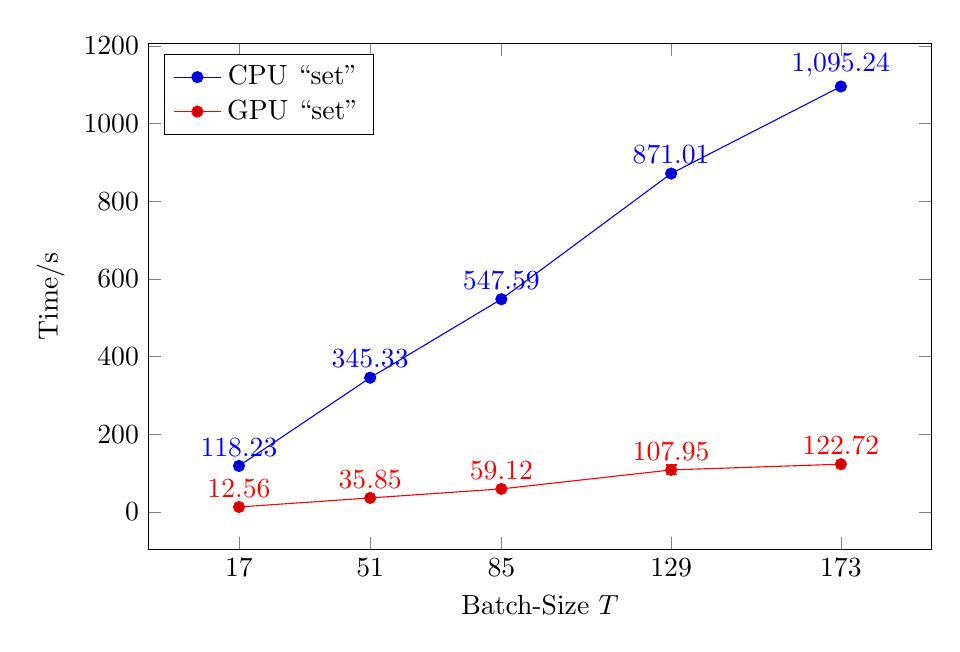
\begin{tikzpicture}
            \begin{axis}[
            width=.95\textwidth,
            height=8cm,
            xtick=data,
            xlabel={Batch-Size $T$},
            ylabel={Time/s},
            enlarge x limits=0.15,
            y tick label style={/pgf/number format/1000 sep=},
            extra y tick style={grid=major, tick label style={xshift=-1cm}},
            legend style={at={(0.02,.98)},
                anchor=north west},
            nodes near coords,
            ]
            \addplot+ [mark=*,error bars/.cd, y dir=both,y explicit] coordinates {
                (17,118.23) +- (1.77, 1.77)
                (51,345.33) +- (2.00, 2.00)
                (85,547.59) +- (1.76, 1.76)
                (129,871.01) +- (3.01, 3.01)
                (173,1095.24) +- (1.71, 1.71)
            };  % cpu
            \addplot+ [mark=*,error bars/.cd, y dir=both,y explicit] coordinates {
                (17,12.56) +- (0.022, 0.022)
                (51,35.85) +- (0.232, 0.232)
                (85,59.12) +- (0.131, 0.131)
                (129,107.95) +- (12.788, 12.788)
                (173,122.72) +- (0.169, 0.169)
            };  % gpu
            \legend{CPU ``set'',GPU ``set''}
            \end{axis}
            \end{tikzpicture}
        \end{subfigure}
        \begin{subfigure}{.4\textwidth}
            \centering
            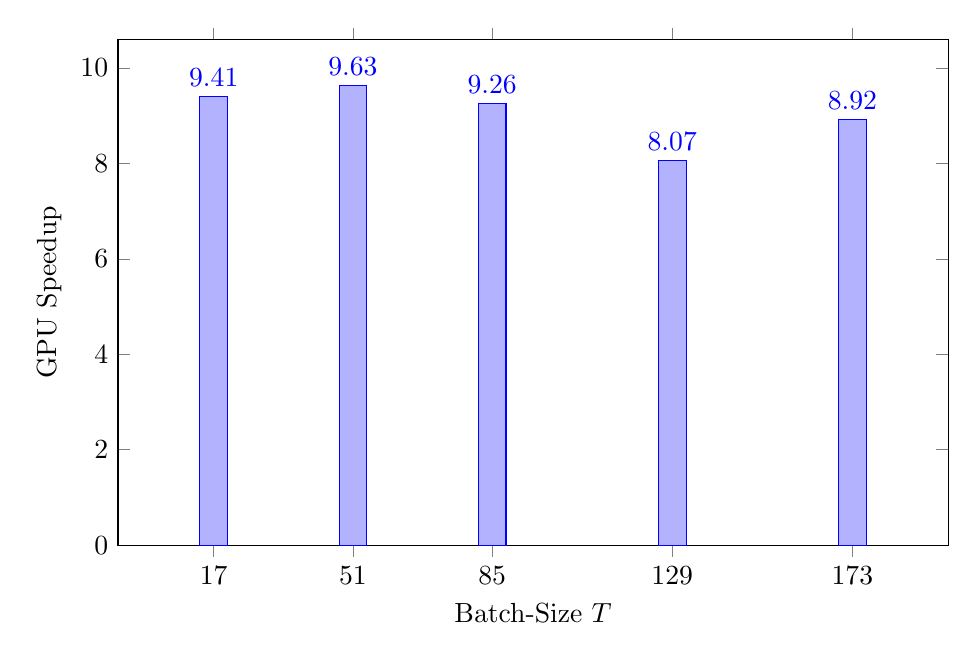
\begin{tikzpicture}
                \begin{axis}[
                ybar,
                width=\textwidth,
                height=8cm,
                xtick=data,
                xlabel={Batch-Size $T$},
                ylabel={GPU Speedup},
                ymin=0,
                enlarge x limits=0.15,
                extra y tick style={grid=major, tick label style={xshift=-1cm}},
                nodes near coords,
                ]
                \addplot+ coordinates {
                    (17,9.41)
                    (51,9.63)
                    (85,9.26)
                    (129,8.07)
                    (173,8.92)
                };
                \legend{}
                \end{axis}
            \end{tikzpicture}
        \end{subfigure}
        \caption[Finding Weights - Execution Times of Different Batch-Sizes $T$ with GPU and CPU ``set'' Separately]{Finding Weights - Execution Times of Different Batch-Sizes $T$ with GPU and CPU ``set'' Separately: The GPU delivers faster computation than CPU even as the datasets' sizes grow - the average speedup is $9.06\pm0.45$. Also, the error bars are indiscernible because they are too small ($< 1\%$)}.
        \label{fig:Execution Times of Different Batch-Sizes with GPU and CPU ``set'' Separately}
    \end{figure}

    \subsection{Pricing Problem's Results} \label{sec:Pricing Problem's Results}
    \subsubsection{Optimization Results} \label{sec:PriProbRes - Optimization}
    Taking the approach mentioned in \Cref{sec:Pricing Problem-Optimizing the Original Dataset}, we obtained consistent loss values for each set of weights (even with differently seeded rewards). The best performing set of weights was set-2, using which the average loss value for the Pricing Problem hovered around $0.0079\%$. Next, running differently seeded rewards with different learning rates on set-2 of weights, we obtained the lowest loss value of $\textbf{0.0068\%}$.
%    \begin{figure}[!htbp]
%        \centering
%        \begin{tikzpicture}
%        \begin{axis}[
%        ybar,
%        width=.6\textwidth,
%        height=7cm,
%        enlarge x limits=0.15,
%        ylabel={Loss Value (in\%)},
%        symbolic x coords={Set-1,Set-2,Set-3,Set-4,Set-5},
%        xtick=data,
%        nodes near coords,
%        nodes near coords align={vertical},
%        xlabel={Models},
%        xlabel style={yshift=-.5cm}
%        ]
%        \addplot+ [error bars/.cd, y dir=both, y explicit] coordinates {
%            (Set-1, 0.0152) +- (0.0001, 0.0001)
%            (Set-2, 0.0079) +- (0.0005, 0.0005)
%            (Set-3, 0.0139) +- (0.0003, 0.0003)
%            (Set-4, 0.0129) +- (0.0002, 0.0002)
%            (Set-5, 0.0155) +- (0.0002, 0.0002)
%        };
%        \end{axis}
%        \end{tikzpicture}
%    \end{figure}

    Compared to the proportional reward distribution (loss values calculated using set-2 of weights), our model's set of rewards produced loss value $\approx$ \textbf{3 times} lower. We again clarify that we compare the best loss values, as the organizer expects to find a distribution that is as optimal as possible.  \Cref{tab:Loss Values Calculated from Different Sets of Rewards} lists the best loss values obtained on each type of reward allocation (model's predicted, random and proportional - \Cref{sec:Pricing Problem-Optimizing the Original Dataset}).
    \begin{table}[!htbp]
        \centering
        \caption[Loss Values Calculated from Different Sets of Rewards]{Loss Values Calculated from Different Sets of Rewards: The values are small because the loss function $Z_P(\vect{r})$ (\Cref{eqn:pricing_problem}) is averaged over the number of locations}
        \label{tab:Loss Values Calculated from Different Sets of Rewards}
        \begin{tabular}{|c|c|}
            \hline
            \textbf{Rewards Obtained From} & \textbf{Best Loss Values (In \%)}\\
            \hline
            Model's Prediction & 0.0068\\
            Random Initialization & 0.0331\\
            Proportional Distribution & 0.0235\\
            \hline
        \end{tabular}
    \end{table}
    
    \subsubsection{GPU Speedup Results} \label{sec:PriProbRes - GPU}
    After running on different batch-sizes $J = 11, 35, 55, 85, 116, 145, 174, 203, 232$, we \textbf{did not observe drastic GPU speedup} for the full model. \Cref{fig:Finding Rewards - Time Taken by the Full Model} shows the Speedup trend: GPU Speedup for the full model was a mere \textbf{1.53 $\pm$ 0.10}.
    \begin{figure}[!htbp]
        \centering
        \begin{subfigure}{\textwidth}
            \centering
            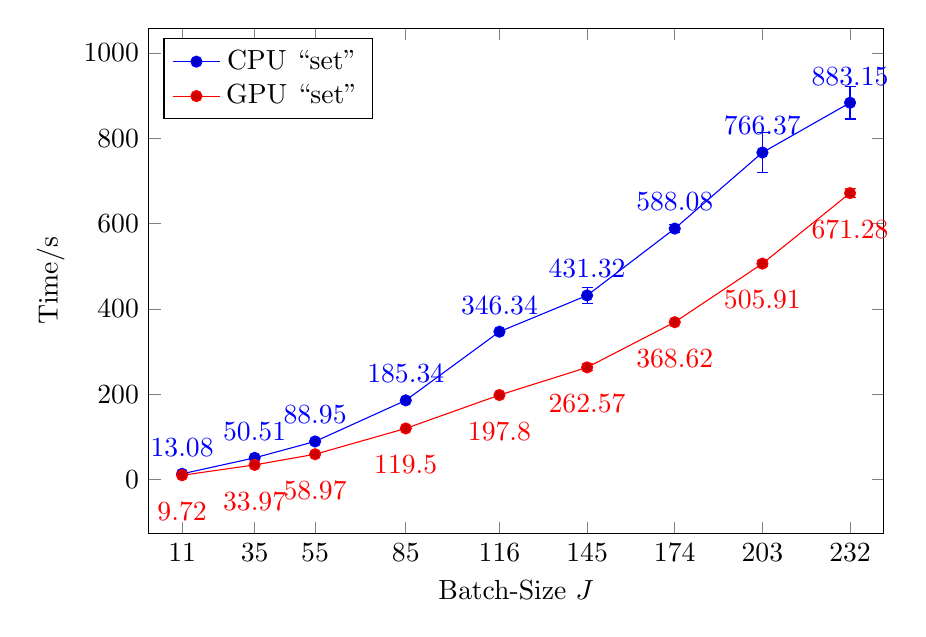
\begin{tikzpicture}
                \begin{axis}[
                width=.9\textwidth,
                height=8cm,
                xtick=data,
                xlabel={Batch-Size $J$},
                ylabel={Time/s},
                enlarge y limits=0.15,
                enlarge x limits=0.05,
                y tick label style={/pgf/number format/1000 sep=},
                extra y tick style={grid=major, tick label style={xshift=-1cm}},
                legend style={at={(0.02,.98)},
                    anchor=north west},
                nodes near coords,
                every node near coord/.append style={yshift=-0.7cm}
                ]
                \addplot+ [mark=*,
                nodes near coords=\raisebox{0.8cm}{\pgfmathprintnumber\pgfplotspointmeta},error bars/.cd, y dir=both,y explicit
                ] coordinates {
                    (11,13.08) +- (1.04, 1.04)
                    (35,50.51) +- (1.73, 1.73)
                    (55,88.95) +- (0.35, 0.35)
                    (85,185.34) +- (0.95, 0.95)
                    (116,346.34) +- (1.67, 1.67)
                    (145,431.32) +- (18.06,18.06)
                    (174,588.08) +- (10.16,10.16)
                    (203,766.37) +- (47.02,47.02)
                    (232,883.15) +- (38.00,38.00)
                };  % cpu
                \addplot+ [mark=*,error bars/.cd, y dir=both,y explicit] coordinates {
                    (11,9.72) +- (0.08, 0.08)
                    (35,33.97) +- (0.26, 0.26)
                    (55,58.97) +- (0.19, 0.19)
                    (85,119.50) +- (0.35, 0.35)
                    (116,197.80) +- (4.02, 4.02)
                    (145,262.57) +- (8.04,8.04)
                    (174,368.62) +- (1.06,1.06)
                    (203,505.91) +- (6.38,6.38)
                    (232,671.28) +- (10.74,10.74)
                };  % gpu
                \legend{CPU ``set'',GPU ``set''}
                \end{axis}
            \end{tikzpicture}
            \caption{Time Taken by the Full Model: GPU Speedup over all batch-sizes is only \textbf{1.53 $\pm$ 0.10}.}
            \label{fig:Finding Rewards - Time Taken by the Full Model}
        \end{subfigure}\vspace*{1em}
        \begin{subfigure}{\textwidth}
            \centering
            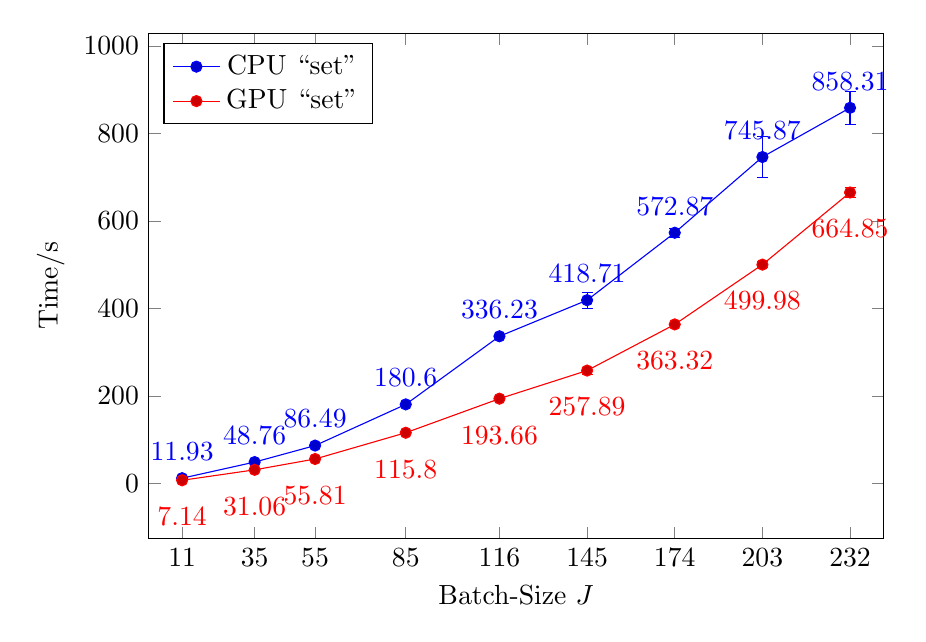
\begin{tikzpicture}
                \begin{axis}[
                width=.9\textwidth,
                height=8cm,
                xtick=data,
                enlarge y limits=0.15,
                enlarge x limits=0.05,
                xlabel={Batch-Size $J$},
                ylabel={Time/s},
                y tick label style={/pgf/number format/1000 sep=},
                legend style={at={(0.02,.98)},
                    anchor=north west},
                nodes near coords,
                every node near coord/.append style={yshift=-0.7cm}
                ]
                \addplot+ [mark=*,
                nodes near coords=\raisebox{0.8cm}{\pgfmathprintnumber\pgfplotspointmeta},error bars/.cd, y dir=both,y explicit
                ] coordinates {
                    (11,11.93) +- (0.94, 0.94)
                    (35,48.76) +- (1.68, 1.68)
                    (55,86.49) +- (0.36, 0.36)
                    (85,180.60) +- (0.97, 0.97)
                    (116,336.23) +- (1.46, 1.46)
                    (145,418.71) +- (18.17,18.17)
                    (174,572.87) +- (10.35,10.35)
                    (203,745.87) +- (46.88,46.88)
                    (232,858.31) +- (37.18,37.18)
                };  % cpu
                \addplot+ [mark=*,error bars/.cd, y dir=both,y explicit] coordinates {
                    (11,7.14) +- (0.08, 0.08)
                    (35,31.06) +- (0.26, 0.26)
                    (55,55.81) +- (0.19, 0.19)
                    (85,115.80) +- (0.35, 0.35)
                    (116,193.66) +- (4.02, 4.02)
                    (145,257.89) +- (8.01,8.01)
                    (174,363.32) +- (1.03,1.03)
                    (203,499.98) +- (6.37,6.37)
                    (232,664.85) +- (10.73,10.73)
                };  % gpu
                \legend{CPU ``set'',GPU ``set''}
                \end{axis}
            \end{tikzpicture}
            \caption[Time taken by the LP]{Time taken by the LP: GPU Speedup over all batch-sizes is only \textbf{1.56 $\pm$ 0.08}. As discussed in \Cref{sec:PriProbRes - GPU,app:Strange GPU Speedup in LP Computation}, we shouldn't have witnessed this speedup as both configurations' LPs were computed on the CPU. Hence, we expected the GPU Speedup value for LP to be $\approx$ 1. }
            \label{fig:Finding Rewards - Time taken by the LP}
        \end{subfigure}
        \caption{Finding Rewards - Execution Times of Different Batch-Sizes $J$ with GPU and CPU ``set'' Separately}
        \label{fig:Finding Rewards - Execution Times of Different Batch-Sizes J with GPU and CPU ``set'' Separately}
    \end{figure}

    Since the the low GPU Speedup was uncanny, we looked for operations that were causing the program to slow down on the GPU. Since the 2-layered network was quite small, we suspected the LP problem (\Cref{eqn:lp_math_constrain_rewards,eqn:lp_code_constrain_rewards}) to influence the runtimes. Thus, we recorded execution times for both the neural network and the LP separately. As we suspected, the LP did impact the runtime more than the neural networks did, and accounted for $\approx 90 \%$ of the total model runtime (\Cref{fig:Finding Rewards - Execution Times of Different Batch-Sizes J with GPU and CPU ``set'' Separately}). However, the GPU Speedup in LP runtime was unusual.
    
    \paragraph{Strange GPU Speedup in LP Computation}
    The Speedup is exceptional as we intentionally transferred the needed matrices/tensors to the CPU for solving the LP using Simplex. SciPy's Optimize Module does not utilize the GPU, and we expected similar runtimes for both configurations. Our efforts to determine the reasons are collected in \Cref{app:Strange GPU Speedup in LP Computation} instead of digressing here. 
    
    We find that the LP in CPU ``set'' was slower than normal because of latency in thread synchronization. Since \Cref{alg:Solving the Pricing Problem} performs operations sequentially (Calculate $loss$ $\rightarrow$ Gradient-Descent and Update $\vect{r}$ Constrain using LP), we think that the CPU performance degrades as it tries to synchronize these steps.
    
    The time elapsed for the Neural Network includes time taken to transfer tensors to and from the GPU, which results in overhead - as seen in higher runtime for lower batch-sizes in Figure \Cref{fig:Finding Rewards - Time taken by the Neural Network}. However, as the batch-sizes grew, we see the computation dominating over the transfer time, resulting in higher CPU ``set'' runtimes; the GPU ``set'' runtimes almost grow linearly for the tested batch-sizes. 

    \begin{figure}[!htbp]
        \centering
        \begin{subfigure}{0.3\textwidth}
            \centering
            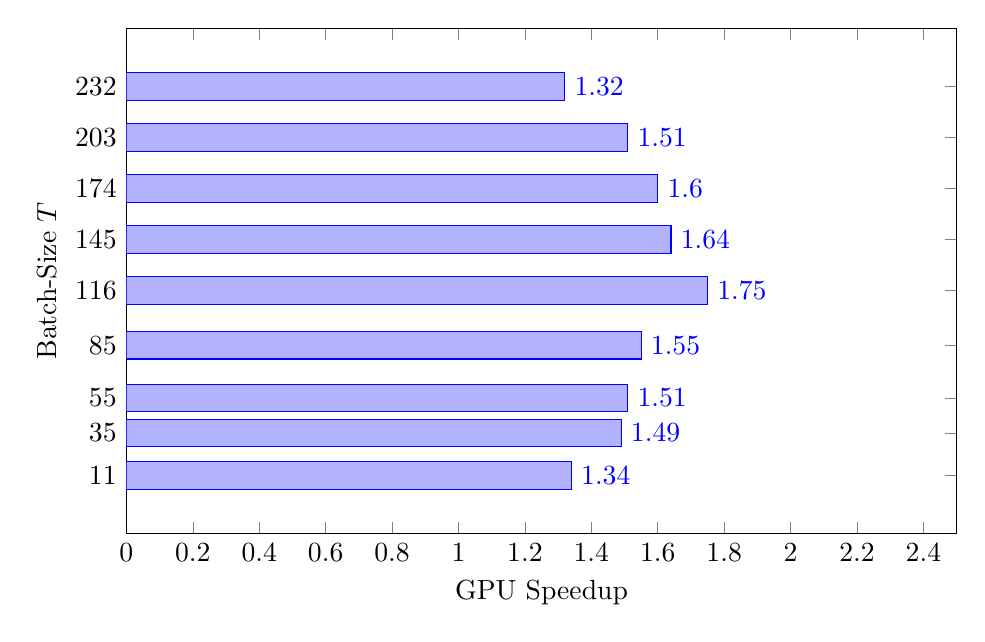
\begin{tikzpicture}
            \begin{axis}[
            xbar,
            width=\textwidth,
            height=8cm,
            ytick=data,
            ylabel={Batch-Size $T$},
            xlabel={GPU Speedup},
            ytick align=inside,
            xmin=0,
            xmax=2.5,
            enlarge y limits=0.15,
            nodes near coords,
            ]
            \addplot+ coordinates {
                (1.34,11)
                (1.49,35)
                (1.51,55)
                (1.55,85)
                (1.75,116)
                (1.64,145)
                (1.60,174)
                (1.51,203)
                (1.32,232)
            };
            \end{axis}
            \end{tikzpicture}
        \end{subfigure}
    \end{figure}
    
    \begin{figure}[!htbp]
        \centering
        \begin{subfigure}{\textwidth}
            \centering
            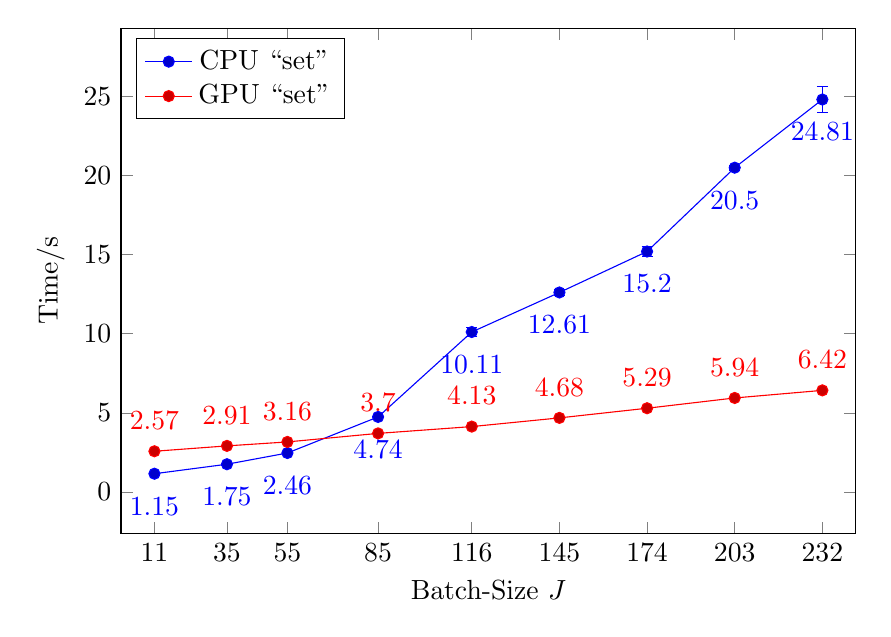
\begin{tikzpicture}
            \begin{axis}[
            width=.9\textwidth,
            height=8cm,
            xtick=data,
            enlarge y limits=0.15,
            enlarge x limits=0.05,
            xlabel={Batch-Size $J$},
            ylabel={Time/s},
            legend style={at={(0.02,.98)},
                anchor=north west},
            nodes near coords,
            every node near coord/.append style={yshift=-0.65cm}
            ]
            \addplot+ [mark=*,error bars/.cd, y dir=both,y explicit] coordinates {
                (11,1.15) +- (0.10, 0.10)
                (35,1.75) +- (0.05, 0.05)
                (55,2.46) +- (0.01, 0.01)
                (85,4.74) +- (0.03, 0.03)
                (116,10.11) +- (0.26, 0.26)
                (145,12.61) +- (0.20,0.20)
                (174,15.20) +- (0.32,0.32)
                (203,20.50) +- (0.15,0.15)
                (232,24.81) +- (0.82,0.82)
            };  % cpu
            \addplot+ [mark=*,
            nodes near coords=\raisebox{0.8cm}{\pgfmathprintnumber\pgfplotspointmeta}, error bars/.cd, y dir=both,y explicit] coordinates {
                (11,2.57) +- (0.01, 0.01)
                (35,2.91) +- (0.01, 0.01)
                (55,3.16) +- (0.01, 0.01)
                (85,3.70) +- (0.004, 0.004)
                (116,4.13) +- (0.001, 0.001)
                (145,4.68) +- (0.03,0.03)
                (174,5.29) +- (0.04,0.04)
                (203,5.94) +- (0.01,0.01)
                (232,6.42) +- (0.01,0.01)
            };  % gpu
            \legend{CPU ``set'',GPU ``set''}
            \end{axis}
            \end{tikzpicture}
            \caption{Time taken by the Neural Network: GPU Speedup over \textit{all} batch-sizes is only \textbf{1.11 $\pm$ 0.60} - mostly due to high transfer times even for low batch-sizes. However, as batch-sizes grow, computation time dominates over transfer time - GPU ``set'' performs better than CPU ``set''.}
            \label{fig:Finding Rewards - Time taken by the Neural Network}
        \end{subfigure}
        \vspace*{1em}
        \caption[Finding Rewards - Execution Times of Different Batch-Sizes $J$ with GPU and CPU ``set'' Separately]{Finding Rewards - Execution Times of Different Batch-Sizes $J$ with GPU and CPU ``set'' Separately: Scaling is strongly hampered by the LP solver. Comparing the contributions of LP and Neural Network to total runtime on GPU ``set'', \textbf{LP accounts for 90.88 $\pm$ 6.95\% of the total time.}}
        \label{fig:Finding Rewards - Execution Times of Different Batch-Sizes J with GPU and CPUa ``set'' Separately}
    \end{figure}
    
    \section{Conclusion} \label{sec:Conclusion}
    Our models for the Identification and the Pricing Problem outperformed previously studied ones \cite{Xue2016Avi2} and other baseline comparisons. For the Identification Problem, the average loss value was 14\% lower than the previous 2-layered model, and 12\% better than the 4-layered model, giving us better results than any other tested model. While we did not test deeper networks, we contend that using more hidden layers will only aggravate overfitting and won't provide better results - as is the case with the 4-layered network. The Pricing Problem's model also delivered at least 3x lower loss values than other baseline comparisons for reward distribution. Clearly, our model outperformed other models in both problems.
    
    On the other hand, we can definitively conclude that the Identification Problem ran faster on the GPU than the CPU, mainly because the model was based on tensors. The Pricing Problem's neural network only performed better with higher batch-sizes, with transfer times hampering performance on lower batch-sizes. With an approximate GPU Speedup of 9.06 for the Identification Problem, we can scale to large datasets more efficiently on the GPU than the CPU. Although the Pricing Problem's model only delivered a speedup of $\approx$ 1.53 (with the LP problem heavily impacting the runtime), the 2-layered network for finding rewards gave a speedup of 1.11 $\pm$ 0.60. (mean over all tested batch-sizes). This shows that neural network are inherently quick to optimize on a GPU, if the batch-sizes are large enough. One can further use a GPU-accelerated LP solver or model the LP in the network itself (if possible) to get faster results. On the other hand, using newer generation GPUs and CPUs can undoubtedly solve the problems faster.
    
    \subsection{Interesting Inferences}
    One may also notice compelling reflections from the results. Although some models perform better than others, they bring out similar, interesting inferences:
    \begin{itemize}
        \item One interesting observation in Table \Cref{tab:Loss Values Calculated from Different Sets of Rewards} is that the Loss Value from the Proportional Distribution (0.161\%) and Random Initialization (0.160\%) are very close, highlighting that the set of weights obtained from the Identification Problem are dependent on other factors ($\matr{f}, \matr{D}$) as well and not just rewards. In other words, incentivizing under-sampled locations more is as good as random distribution of rewards - as agents don't get more heavily influenced by rewards than any other factor to visit locations.\\
        Moreover, by looking at the model's generated rewards, one can infer that the model chooses to place large rewards in 
    \end{itemize}

    \subsection{Further Research}
    There exist numerous possibilities for solving the problems better and faster - from more complex models to better preprocessing. Some important suggestions are listed below:
    
    \paragraph{Choice of Gradient-Descent Algorithm} Figure \Cref{fig:Plot for 3-layered Model} shows how the choice of Adam's algorithm \cite{Adam} for \textsc{Gradient-Descent}($\cdot$) helps the model to learn quickly. However, we also witness long periods of saturation after few epochs. This was the case for several other algorithms (SGD \cite{SGD} and Adagrad \cite{Adagrad}), but with different paces of learning. Since the organizers would want to further optimize the set of weights even, research could be done on avoiding the long, unchanging saturation phase. This may involve using other techniques for \textsc{Gradient-Descent}($\cdot$) (Algorithm \Cref{alg:Algorithm for the Identification Problem}) and/or altering the loss function $Z_P(\matr{w_1}, \matr{w_2})$ (Equation \Cref{eqn:iden_problem}).
    
    \paragraph{Modeling LP Differently to Reduce Runtimes} LP is a simple tool for optimizing different problems, with various algorithms for solving LPs - Simplex, Criss-Cross and other Interior Point techniques. While it gives optimal results, it can be computationally expensive if the matrices are large (as depicted in Figure \Cref{fig:Finding Rewards - Time taken by the LP}). One can try several approaches to reduce computation time here:
    \begin{itemize}
        \item Implement GPU Support for the LP. Good CUDA backend support did not exist during our study, forcing us to use SciPy's Optimize Module, which only supported NumPy matrices on the CPU.
        \item Constrain Rewards differently (\Cref{sec:Constraining Rewards}). We were unsuccessful in implementing a dual version of the LP, interspersed with the neural network. Nonetheless, constraining rewards using a neural network would drastically improve performance as the current LP accounts for $\approx$ 90\% of the total runtime.
    \end{itemize}

    \bibliographystyle{IEEEtran}
    \bibliography{IEEEabrv,avicaching}
    
    \cleardoublepage
    \begin{appendices}
    \section{Implementation} \label{sec:Implementation}
    The code can be found here[]. \\
    Both the Identification and the Pricing Problem were programmed in Python 2.7 using NumPy 1.12.1, SciPy 0.19.1 and PyTorch 0.1.12 modules [web cites] \cite{SCPOptimizeDocs}\cite{NPDocs}. [Results from Python plotted in Matplotlib 2.0.2] With some code optimizations, the input dataset $\matr{F}$ was built using NumPy's \texttt{ndarray} and PyTorch's \texttt{tensor} functions. Since PyTorch offers NumPy-like code base but with dedicated neural network functions and submodules, PyTorch's \texttt{relu} and \texttt{softmax} functions were used along with other matrix operations.\\
    
    \subsection{Specific Implementation Details for the Pricing Problem}
    Among all the code optimizations in both models, some in that for the Pricing Problem are worth discussing, as they drastically differ from Algorithm \ref{alg:Solving the Pricing Problem} or are intricate. Most optimizations relevant to the Identification Problem are trivial and relate directly to those for the Pricing Problem. Therefore, only those in the Pricing Problem model are discussed.
    
    \subsubsection{Building the Dataset $\matr{F}$}
    Notice that we build the dataset $\matr{F}$ and batch-multiply it with $\matr{w_1}$ on each iteration/epoch (lines 2-3 of Algorithm \ref{alg:Solving the Pricing Problem}). Doing these steps are repetitive as most elements of $\matr{F}$, distances $\matr{D}$ and environmental feature vector $\vect{f}$, do not change unlike rewards $\vect{r}$. Moreover since $\matr{w_1}$ is fixed, Algorithm \ref{alg:Solving the Pricing Problem} would repetitively multiply the $\vect{f}$ and $\matr{D}$ components of $\matr{F}$ with $\matr{w_1}$. To avoid these unnecessary computations, we preprocessed most of $\matr{F}$ by batch-multiplying with $\matr{w_1}$ and only multiplied $\vect{r}$ with the corresponding elements of $\matr{w_1}$. Figure \ref{fig:Splitting and Batch Multiplying F and w1} describes the process graphically.\\
    \begin{figure}[!htbp]
        \centering
        \includegraphics[width=\linewidth]{split_and_batch_multiply}
        \caption{Splitting and Batch Multiplying $\matr{F}$ and $\matr{w_1}$}
        \label{fig:Splitting and Batch Multiplying F and w1}
    \end{figure}    
    Although this preprocessing might seem applicable for the model in Identification Problem too, it does not apply fully. Since the weights $\matr{w_1}$ are updated on each iteration/epoch, we cannot multiply them with parts of $\matr{F}$ beforehand (Algorithm \ref{alg:Algorithm for the Identification Problem}). However, we can combine $\matr{D}$ and $\vect{f}$ in the preprocessing stage and simply append $\vect{r}[t]$ on each iteration, saving computation time.
    
    \subsubsection{Modeling the Linear Programming Problem in the Standard Format}
    The \texttt{scipy.optimize} module's \texttt{linprog} function requires that the arguments are in standard LP format. As discussed in \cref{sec:Calculating Rewards}, Equation \ref{eq:lp_code_constrain_rewards} resembles the standard format more closely than \ref{eq:lp_math_constrain_rewards}, but it may not be clear how so.\\
    
    Considering $\vect{u}$ and $\vect{r'}$ as variables $\vect{x}$, Equation \ref{eq:lp_code_constrain_rewards} translates into Equation \ref{eq:lp_matrix_rewards} ($J$ is the number of locations).
    \begin{equation} \label{eq:lp_matrix_rewards}
    \begin{aligned}
    & \text{minimize}
    & & \begin{bmatrix}
    \vect{0_J}\\
    \vect{1_J}\\
    \end{bmatrix}^T
    \begin{bmatrix}
    \vect{r'}\\
    \vect{u}
    \end{bmatrix}\\ \\
    & \text{subject to}
    & & \begin{bmatrix}
    I_J & -I_J\\
    -I_J & -I_J\\
    \vect{1}^T_J & \vect{0}^T_J\\
    \end{bmatrix}
    \begin{bmatrix}
    \vect{r'}\\
    \vect{u}\\
    \end{bmatrix} \leq
    \begin{bmatrix}
    \vect{r}\\
    -\vect{r}\\
    \mathcal{R}\\
    \end{bmatrix}\\
    &&& r'_i, u_i \geq 0
    \end{aligned}
    \end{equation}
    
    \section{Strange GPU Speedup in LP Computation} \label{sec:Strange GPU Speedup in LP Computation}
    Even though we intentionally transferred the rewards vector to and constrained it using \texttt{scipy.optimize} module's \texttt{linprog} function on the CPU, we obtained an unexpected GPU speedup in the runtimes (see \cref{sec:PriProbRes - GPU} and Figure \ref{fig:Finding Rewards - Time taken by the LP}). Confounded by this weird behavior, we wanted to pinpoint the reasons because SciPy's function could not have differentiated between the configurations and delivered different results. However, since this was not our research's prime motive, we did not take a strong quantitative approach in determining the cause(s). There could have been many reasons for this bizarre behavior, including but not limited to:
    \begin{enumerate}
        \item SciPy's Optimize Module differentiating between configurations. This can be ruled out because the module could not have known the configuration during which it was called. This is because the configuration settings were applicable only on user-programmed operations, and needed to be explicitly stated - as mandated by PyTorch \cite{PTDocs}. SciPy's Optimize Module identifying the configurations is just supernatural.
        \item CPU ``set'' using exploiting more main memory than GPU ``set''. We suspected that since CPU ``set'' configuration's operations were executed solely on the CPU, the residing datasets could have used more main memory than when GPU ``set'' was running. This could have hampered the performance of LP with CPU ``set''. Unlike the 1\textsuperscript{st} possibility, this would have meant that CPU ``set'' was slowing down the LP, and not that GPU ``set'' was speeding up the LP.
    \end{enumerate}

    The 2\textsuperscript{nd} hypothesis/possibility seemed more promising than the others, and we built some programs to test its various aspects, which are elaborated in next sections.
    
    \subsection{Main Memory Usage by Both Configurations}
    As the initial approach, we logged details of main memory usage when the models were running. Contrary to our expectations (again), the GPU ``set'' was utilizing more main memory than CPU ``set'' was. Precisely, when running the Pricing Problem's model with $T = 173, J = 116$ without GUI and logging at 0.2 second intervals until the model completed, the GPU ``set'' was using 9.0 - 9.1 \% of the main memory, whereas CPU ``set'' was using only 0.9 \% memory. During the tests, only 1 CPU core was utilized for GPU ``set'', whereas 6-8 cores were being used for CPU ``set''. Clearly, main memory usage wouldn't have been the reason for the strange GPU speedup in LP runtime as LP's GPU ``set'' runtime would have been lower if the relation with main memory usage was true. However, there could be a relation between CPU usage and LP runtime.
    
    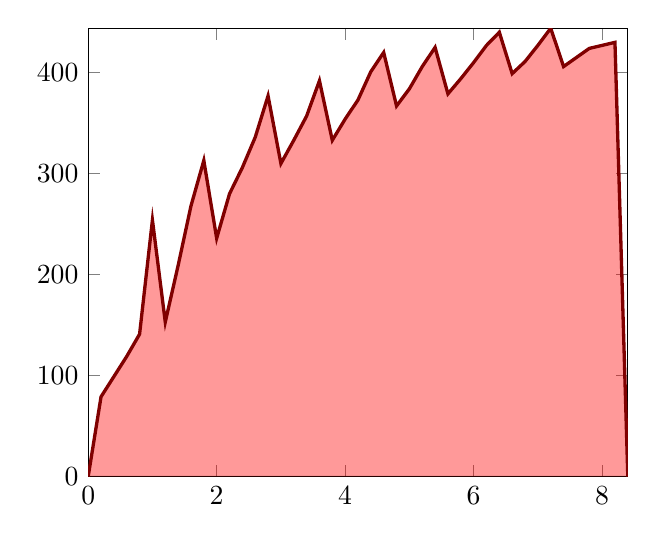
\begin{tikzpicture}
    \begin{axis}[
    domain=0:10,
    enlargelimits=false,
    ]
    %
    \addplot[fill=red, opacity=.4, domain=0:10] coordinates {
        (0.0, 0)
        (0.2, 79.0)
        (0.4, 99.0)
        (0.6, 119)
        (0.8, 141)
        (1.0, 254)
        (1.2, 153)
        (1.4, 209)
        (1.6, 268)
        (1.8, 313)
        (2.0, 236)
        (2.2, 280)
        (2.4, 306)
        (2.6, 336)
        (2.8, 377)
        (3.0, 310)
        (3.2, 333)
        (3.4, 357)
        (3.6, 392)
        (3.8, 333)
        (4.0, 354)
        (4.2, 373)
        (4.4, 401)
        (4.6, 420)
        (4.8, 367)
        (5.0, 384)
        (5.2, 406)
        (5.4, 425)
        (5.6, 379)
        (5.8, 394)
        (6.0, 410)
        (6.2, 427)
        (6.4, 440)
        (6.6, 399)
        (6.8, 411)
        (7.0, 427)
        (7.2, 444)
        (7.4, 406)
        (7.6, 415)
        (7.8, 424)
        (8.0, 427)
        (8.2, 430)
        (8.4, 0)
    }\closedcycle;
    
    \addplot [very thick, red!50!black] coordinates {
        (0.0, 0)
        (0.2, 79.0)
        (0.4, 99.0)
        (0.6, 119)
        (0.8, 141)
        (1.0, 254)
        (1.2, 153)
        (1.4, 209)
        (1.6, 268)
        (1.8, 313)
        (2.0, 236)
        (2.2, 280)
        (2.4, 306)
        (2.6, 336)
        (2.8, 377)
        (3.0, 310)
        (3.2, 333)
        (3.4, 357)
        (3.6, 392)
        (3.8, 333)
        (4.0, 354)
        (4.2, 373)
        (4.4, 401)
        (4.6, 420)
        (4.8, 367)
        (5.0, 384)
        (5.2, 406)
        (5.4, 425)
        (5.6, 379)
        (5.8, 394)
        (6.0, 410)
        (6.2, 427)
        (6.4, 440)
        (6.6, 399)
        (6.8, 411)
        (7.0, 427)
        (7.2, 444)
        (7.4, 406)
        (7.6, 415)
        (7.8, 424)
        (8.0, 427)
        (8.2, 430)
        (8.4, 0)
    };
    \end{axis}
    \end{tikzpicture}
    
    \subsubsection{asdf}
\end{appendices}
\end{document}